\section{Gaussian Multiple-Access Channels}
This is the continuation of subsection \ref{sec 6.2} but with more details. We start with two senders, $X_1$ and $X_2$, who communicate to the single receiver, $Y$. The received signal at time $i$ is
%
\begin{eqnarray}
    Y_i = X_{1i}+X_{2i}+Z_i,
\end{eqnarray}
%
where $\{Z_i\}$ is a sequence of i.i.d., zero mean Gaussian random variables with variance $N$ as shown in figure \ref{fig:GMAC}.
%
\begin{figure}[h]
    \centering
    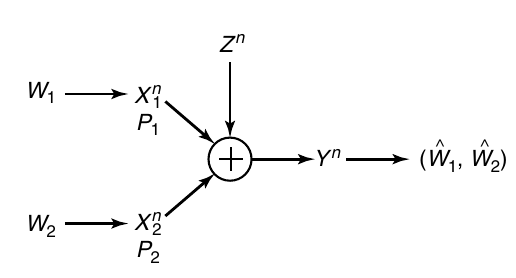
\includegraphics[scale=0.40]{Diagrams/GMAC.png}
    \caption{Gaussian Multiple-access channel with two senders and single receiver}
    \label{fig:GMAC}
\end{figure}
%
Here, we have different power constraints for different senders. We consider $P_j$ be the power constraint associated with the sender $j$, \textit{i.e.} for each sender and all messages we must have,
%
\begin{eqnarray}
    \frac{1}{n} \sum_{i = 1}^n x^2_{ij} (w_j) \leq P_j, \quad w_j \in \{1,2,...,2^{nR_j}\}, \quad j = 1,2.
\end{eqnarray}
%
The Gaussian channel was included in the proof of achievability of channel capacity for the discrete case. The proof can also be extended. Likewise, the converse may be extended. The convex hull of the set of rate pairings meeting \eqref{8.4.1} for some input distribution $f_1(x_1)f_2(x_2)$ satisfying $\expt{X_1^2} \leq P_1$ and $\expt{X_2^2} \leq P_2$ is, thus, the capacity area. 
%%%%
\subsection{Gaussian multiple-access channel Capacity Pentagon}
Let us also draw the capacity pentagon for the Gaussian multiple-access channel. Let us expand the mutual information in terms of relative entropy \textit{i.e.}
%
\begin{eqnarray}
    I(X_1;Y|X_2) &=& h(Y|X_2) - h(Y|X_1,X_2) \nonumber\\
    &=& h(X_1+X_2+Z|X_2) - h(X_1+X_2+Z|X_1,X_2) \nonumber\\
    &=& h(X_1+Z|X_2) - h(Z|X_1,X_2) \nonumber\\
    &=& h(X_1+Z|X_2) - h(Z) \quad \text{[As $Z$ is independent of $X_1$ and $X_2$]} \nonumber\\
    &=& h(X_1+Z) - h(Z) \quad \text{[$X_1$ and $X_2$ is independent]} \nonumber\\
    &=& h(X_1+Z) - \frac{1}{2}\log(2\pi e)N \nonumber\\
    &\leq& \frac{1}{2}\log(2\pi e)(P_1+N) - \frac{1}{2}\log(2\pi e)N \quad \text{[The normal maximizes entropy for a given second moment]} \nonumber\\
    &=& \frac{1}{2}\log(1+\frac{P_1}{N})
\end{eqnarray}
%
Thus, the maximizing distribution is $X_1 \sim \mathcal{N}(0,P_1)$ and $X_2 \sim \mathcal{N}(0,P_2)$ with $X_1$ and $X_2$ independent. Similarly,
%
\begin{eqnarray}
    I(X_2;Y|X_1) \leq \frac{1}{2}\log(1+\frac{P_1}{N})
\end{eqnarray}
%
Now, let us calculate $I(X_1;Y)$. 
%
\begin{eqnarray}
   I(X_1;Y) &=& h(Y)-h(Y|X_1) \nonumber\\
   &=& h(X_1+X_2+Z)-h(Y|X_1) \nonumber\\
   &=& h(X_1+X_2+Z)-h(X_1+X_2+Z|X_1) \nonumber\\
   &=& h(X_1+X_2+Z)-h(X_2+Z|X_1) \nonumber\\
   &\leq& \frac{1}{2}\log(2\pi e)(P_1+P_2+N)-\frac{1}{2}\log(2\pi e)(P_2+N) \nonumber\\
   &=& \frac{1}{2}\log\lrfb{\frac{P_1+P_2+N}{P_2+N}} \nonumber\\
   &=& \frac{1}{2}\log\lrfb{1+\frac{P_1}{P_2+N}} \nonumber\\
\end{eqnarray}
%
Again the equality is achieved when the distribution is $X_1 \sim \mathcal{N}(0,P_1)$ with $X_1$ and $X_2$ independent. Similarly,
%
\begin{eqnarray}
    I(X_2;Y) \leq \frac{1}{2}\log\lrfb{1+\frac{P_2}{P_1+N}} 
\end{eqnarray}
%%
The distribution simultaneously maximizes the mutual information bounds in \eqref{8.4.1}. 
%
\begin{tcolorbox}[boxrule=0pt,frame hidden,sharp corners,enhanced, opacityback=0, borderline west={2pt}{0pt}{red}]
\begin{defn} \textbf{(Channel Capacity Function)} The channel capacity function corresponding to the channel capacity of a Gaussian white-noise channel with signal-to-noise ratio $x$ is
%
\begin{eqnarray}
    C(x) := \frac{1}{2}\log(1+x)
\end{eqnarray}
%
\end{defn}
\end{tcolorbox}
%
Therefore the bound on $R_1$, $R_2$ and $R_1+R_2$ as
%
\begin{eqnarray}
    R_1 &\leq& C\lrfb{\frac{P_1}{N}} \\
    R_2 &\leq& C\lrfb{\frac{P_2}{N}} \\
    R_1+R_2 &\leq& C\lrfb{\frac{P_1+P_2}{N}}.
\end{eqnarray}
%
Equality is achieved when $X_1 \sim \mathcal{N}(0,P_1)$ and $X_2 \sim \mathcal{N}(0,P_2)$ and define the capacity region. The diagram is shown in the figure \ref{fig:GMACC}.
%
\begin{figure}[h]
    \centering
    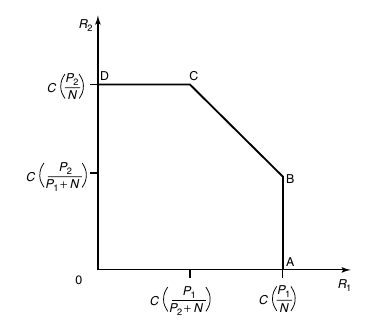
\includegraphics[scale=0.40]{Diagrams/GMACC.png}
    \caption{Gaussian Multiple-access channel capacity}
    \label{fig:GMACC}
\end{figure}
%
In this case, the most exciting and surprising fact is that the sum of the rates can be as large as $C(\frac{P_1+P_2}{N})$, which is that rate achieved by a single transmitter sending with a power equal to the sum of the powers.
%%%%%%
\subsubsection*{Interpretation of Corner points}
The interpretation is almost equivalent to the case described for a general multiple-access channel for a fixed distribution. Consider the decoding as a two-stage process:
\begin{enumerate}
    \item  \textbf{The First Stage:} The receiver decodes the second sender, considering the first sender as a part of the noise with a low probability of error if $R_2 < C(\frac{P_2}{P_1+N})$.

    \item \textbf{The Second Stage:} After the second sender is decoded successfully, it can be subtracted out, and the first sender can be decoded correctly if $R_1 < C(\frac{P_1}{N})$. 
\end{enumerate}
%
Therefore, we can achieve the rate pairs at the corner points of the capacity region utilizing single-user operations. This process is known as \textit{onion-peeling}, and it can be extended to any number of users. \\ 
For $m$ senders with equal power, the total rate is $C(\frac{mP}{N})$ and the average rate per sender is 
%
\begin{eqnarray}
    \frac{\langle R \rangle}{m}= \frac{1}{m}C\lrfb{\frac{mP}{N}}
\end{eqnarray}
%
As $m \rightarrow \infty$, the total rate $C(\frac{mP}{N}) \rightarrow \infty$ and $\frac{\langle R \rangle}{m} \rightarrow 0$. This proves there is a lot of interference if there are a lot of senders overall. However, even if the rate per individual sender drops to zero, we may still communicate an infinitely huge quantity of information overall.
%
\begin{tcolorbox}[enhanced,
  colback=green!0!black!0!white,colframe=black!15!blue,title=\textbf{Code-Divison Multiple-Access (CDMA)}]
The capacity region described above, where separate codes are used for the different senders, and the receiver decodes them individually, belongs to Code-Divison Multiple-Access (CDMA).
\end{tcolorbox}
%

\subsection{Equivalent of Gauss's Law}
For a Gaussian multiple-access system with $m$ sources with powers $P_1, P_2,..., P_m$ and the ambient noise of power $N$, we can state the equivalent of Gauss's law for any set $S$ in the form,
%
\begin{eqnarray}
    \text{Total rate of information flow from $S$ } = \sum_{i \in S}R_i \leq C\lrfb{\frac{\sum_{i\in S} P_i }{N}}. 
\end{eqnarray}